%% abtex2-modelo-include-comandos.tex, v-1.9.2 laurocesar
%% Copyright 2012-2014 by abnTeX2 group at http://abntex2.googlecode.com/ 
%%
%% This work may be distributed and/or modified under the
%% conditions of the LaTeX Project Public License, either version 1.3
%% of this license or (at your option) any later version.
%% The latest version of this license is in
%%   http://www.latex-project.org/lppl.txt
%% and version 1.3 or later is part of all distributions of LaTeX
%% version 2005/12/01 or later.
%%
%% This work has the LPPL maintenance status `maintained'.
%% 
%% The Current Maintainer of this work is the abnTeX2 team, led
%% by Lauro César Araujo. Further information are available on 
%% http://abntex2.googlecode.com/
%%
%% This work consists of the files abntex2-modelo-include-comandos.tex
%% and abntex2-modelo-img-marca.pdf
%%

% ---
% Este capítulo, utilizado por diferentes exemplos do abnTeX2, ilustra o uso de
% comandos do abnTeX2 e de LaTeX.
% ---
\documentclass[
12pt, 
a4paper,
oneside,			% para impressão em verso e anverso. Oposto a oneside
english,			% idioma adicional para hifenização
french,				% idioma adicional para hifenização
spanish,			% idioma adicional para hifenização
brazil,	
]{abntex2}
\usepackage[boxed,linesnumbered]{algorithm2e}
\usepackage{lmodern}	
\usepackage[T1]{fontenc}		% Selecao de codigos de fonte.
\usepackage[utf8]{inputenc}
\usepackage{microtype}
\usepackage[brazilian]{backref}
\usepackage{indentfirst}
\usepackage{color}
\usepackage{graphicx}			% Inclusão de gráficos

\instituicao{Faculdades de Ciencias e Tecnologia de Montes Claros -- FACIT
	\par
	Engenharia da Computação
	\par
	Inteligencia Computacional}
\titulo{Relatório Perceptron}
\author{Leonardo Vieira Guimarães}
\local{Montes Claros}
\date{Outubro 2014}
\tipotrabalho{Relatório Perceptron}
\preambulo{Implementar o Perceptron utilizando a linguagem Python}
% O tamanho do parágrafo é dado por:
\setlength{\parindent}{1.0cm}


\begin{document}
	% Capa
	\imprimircapa
	% Folha de rosto
	\imprimirfolhaderosto
	
	% inserir o sumario
	% ---
	\pdfbookmark[0]{\contentsname}{toc}
	\tableofcontents*
	\cleardoublepage
	% ---
	\textual

	%Introdução
	
	\chapter*[INTRODUÇÃO]{INTRODUÇÃO}
	\addcontentsline{toc}{chapter}{INTRODUÇÃO}
	
	Este trabalho tem como objetivo a utilização de ferramenta computacional para a implementação do Perceptron, que neste caso foi usado a linguagem python, com as bibliotecas Numpy, matplotlib.pyplot, o math e o \_\_future\_\_ division. 	
	
	A implementação do perceptron utilizou uma classe que encapsulou as funções de treinamento, execução e validação. Foram utilizadas algumas funções do Numpy que facilitou a implementação do algoritmo na diminuição dos FOR e na manipulação de matrizes. Nesta mesma estrutura foram inseridas  duas funções, uma para a plotagem do gráfico de erro e a outra para a plotagem do gráfico de pesos. Todas as funções foram explicadas e comentadas no corpo do algoritmo. E os resultados obtidos dos erros e pesos foram salvos nos arquivos ErrosEpocas.txt e Pesos.txt na pasta arquivos. 
	
	O Numpy e uma biblioteca para computação científica que utiliza a linguagem Python, podendo manipular álgebra linear, transformada de Fourier, números aleatórios, matriz N-dimensional e entre outras funções. \cite{python}
	
	O matplotlib.pyplot e uma biblioteca que contém funções para manipulação de gráficos e algumas tipos de imagens.
	
	O math é uma biblioteca que contém funções matemáticas com raiz quadrada, exponencial entre outros. Por fim o \_\_future\_\_ division é uma função que possibilita a obtenção de um tipo float para divisão de dois números qualquer. 
	
	Foi utilizado o linguagem de programação Phyton 2.7 que possui estrutura de dados de alto nível, adota uma abordagem simples efetiva para programação orientadas a objeto, com natureza interpretada, distribuição livre, tendo extensa variedades de bibliotecas e entre outras funções. A linguagem já veio instalado no PythonXY, ferramenta que vem embutido com alguns IDEs (neste trabalho foi utilizado o Spyder), bibliotecas, console python e entre outras funções.   
	
	Os objetivos específicos deste trabalho foram divididos em dois problemas:
	
	O primeiro problema, Separação de Duas Classes Bidimensionais, foi reescrever a função Gaussclass.m escrito em Matlab para Python, utilizando as funções tile e randn do modulo Numpy. 
	
	Neste problema deve-se gerar testes com duas classes de amostras, com e sem superposição. Com os resultados obtidos de pessos e eros, foram gerados dois gráficos, um com a reta de separação e as classes e a  e o outro com os erros quadrado médio por cada época, isso feito para cada teste. Não foi pedido o conceito de validação para esta questão porém caso o usuário deseje ver o percentual de validação pode estar executando. 
	
	O segundo problema, Diagnóstico de Doença Cardíaca, contém um arquivo heart.txt com 270 amostras e 14 parâmetros, sendo a ultima coluna classificada como o  tipo de classe que podemos chamar de valor esperado, sendo o valor 1 ausência da doença e o valor 2 presença da doença cardíaca. O restante dos parâmetros são respectivamente idade, sexo, tipo de dor no peito, pressão arterial, colesterol, açúcar no sangue, eletrocardiograma, frequência cardíaca, exercício, relação de exercício, repouso, inclinação do pico de exercício, números de calorias e o thal.
	
	Foram realizados alguns testes obtendo o percentual de  validação e o gráfico de erro quadrado médio para cada época. Sendo que os valores de pesos e os erros foram salvos nos arquivos Pesos.txt e ErrosEpocas.txt respectivamente. O algoritmo DadosHeart.m escrito em Matlab foi reescrito em Python, sendo este ultimo como questão bônus.  
	
		
	\chapter{DESENVOLVIMENTO}
	O Perceptron e basicamente um tipo de estrutura de dados para estudar uma rede neural, inserindo o conceito de aprendizagem baseado no modelo de um neurônio artificial. Com as entradas (amostras) e os os pesos das conexões e realizado uma junção somadora, na qual se realiza uma função de ativação f(u) obtendo uma saída de ativação y, sendo u uma saída linear.  
	
	Para construção do perceptron foi necessário o entendimento das equações mostradas a seguir que foram utilizadas para implementação do perceptron. \cite{perceptron}\cite{redes}
	
	
	
	\begin{equation}
	y = f(u) = f(\sum_{j = 1}^{m} W_{j}X_{j}) = \left\{\begin{array}{rc}
	1,&\mbox{se}\quad u\le 0,\\ 0, &\mbox{se}\quad u>0.
	\end{array}\right.
	\end{equation}
	

	
	
	\begin{equation}
	w_{1}x_{1}+w_{2}x_{2}+...+w_{m}x_{m} = \theta \Rightarrow w_{1}x_{1}+w_{2}x_{2}+...+w_{m}x_{m} - \theta = 0
	\end{equation}
	
	\begin{equation}
	W_{k+1} = W_{k} + \eta e X_{k}
	\end{equation}
	
	\begin{itemize}
		\item u saída linear 
		\item y saída de ativação
		\item n taxa de aprendizagem
		\item e erro = Saída desejada(d) - Saída obtida(y) 
		\item X padrão de entrada
	\end{itemize}
	
	
	
	Na implementação usamos as bibliotecas numpy, numpy.raandom, matplotlib.pyplot e math. Foi criada uma classe perceptron que encapsulo as funções execução, treinamento, validação, ploterro e plotretapesso. 
	
	No numpy foram utilizados as funções matrix, arange, concatenate, loadtxt, amax, numpy.random, random\_sample e o shuffle. Com matplotlib.pyplot usamos as funções figure, xlabe, ylabel, grid, ylim, xlim, plot, savefig e show.
	
	Na função de execução recebe a entrada x determinada por cada coluna de uma matriz de amostras que é multiplica com os pesos w sendo que o resultado é igual a matriz u. Com o resultado obtido realiza-se a saída de ativação y, onde se u for maior ou igual a zero y é igual a 1, caso contrario y é igual a zero. \\
	
	def execucao(self, x):
	
    \setlength{\parindent}{1,5 cm}
    
		 x = matrix(x) 
		        
		 u = matrix(self.w)*x\
		
		 u = u[0,0]
		           
		 if u >= 0:
		
		\hspace{0,5cm}y = 1
		
		if u < 0:
		
		\hspace{0,5cm}y = 0
		
	     return y\\
	     
	     \setlength{\parindent}{1,0 cm}
	
	A função validação recebe as amostras x e os valores esperados. Inicializa a lista de obtido y e a lista do bias sendo os dois  referente ao tamanho da amostra e valores 0 e -1 respectivamente, para isso foi utilizando a função len que retorna a quantidade de elementos de uma lista. 
	
	Em seguia realiza-se a concatenação das amostras com os bias, converte a lista em uma matriz, chama a função execução para cada amostra e salva uma vetor yvalidacao e imprime alguns resultados.
	
	def validacao(self, xvalidacao, d): 
	
	\setlength{\parindent}{1,5 cm}
	  
	yvalidacao = [0]*len(xvalidacao[0])
	
	bias = [-1]*len(xvalidacao[0])
	
	xvalidacao = concatenate((xvalidacao,[bias]), axis=0) 
	     
	xvalidacao = matrix(xvalidacao)
	
	cont = 0 
		
	for j in range(0,len(yvalidacao)): 
		
		\hspace{0,5cm}yvalidacao[j] = self.execucao(xvalidacao[0:len(xvalidacao),j])
		
		\hspace{0,5cm}if yvalidacao[j] == d[j]:
		
		\hspace{1,0cm}cont = cont + 1   
		  
	    print "valores validaddos---------", yvalidacao 
		
	    print "Porcentagem de validacao---",(cont/len(yvalidacao))*100 
		 
	    return yvalidacao\\
	    
	    \setlength{\parindent}{1.0 cm}

 A função treinamento recebe as amostras, o valor esperado e a quantidade máxima de iterações. Inicializa a taxa de aprendizagem que como padrão tem o valor de 0,01, as listas de valor desejado y, o erro e os psesos aleatórios entre 0 e 1 que utiliza a função random\_sample para gerar esses valores. 
 
 Os pesos quando iniciam aleatoriamente entre 0 e 1 podemos obter uma variedades de resultados. Quando se coloca os pesos iguais a zero encontrávamos somente um resultado. 
 
 Sendo p uma variável que recebe uma lista de números inteiro de 0 até a quantidade de amostras aleatoriamente. Para a obtenção de p usamos a função len que conta a quantidade de elementos contidos em um lista e com o função arange que monta a lista de 0 ate o valor que o len obteve. Em seguida com a lista de p definida ocorreu a mistura aleatória de seus valores, para isso utilizamos a função shuffle que realiza a mistura dos valores de forma aleatório. Sendo que nesta parte da função de treinamento ocorre a aleatoriedade das amostras. 
 
 A função for terá o valor aleatória das entradas ou amostras, onde irá chamar a função de execução que fará a verificação do valor obtido retornado 1 ou 0, com esse valor obtém-se o erro, assim sendo possível fazer os ajustes dos pesos. 
 
 Se o erro for diferente de zero ocorrerá os ajustes dos pesos, caso contrario os pesos não terão alterações, esse processo irá terminar ate que se encontre todos os valores desejados igual ao obtido ou até a finalização do loop determinado pelo usuário. No treinamento também foi inserido as funções de manipulação de arquivos, salvando os pesos e os erros obtidos e imprimindo alguns resultados. 
 

def treinamento(self, x, d, q):

\hspace{1,5cm}errosepocas = open("arquivos/ErrosEpocas.txt","w") 

\hspace{1,5cm}pesos = open("arquivos/Pesos.txt","w")

\hspace{1,5cm}self.x = x

\hspace{1,5cm}n = 0.01

\hspace{1,5cm}bias = [-1]*len(d)

\hspace{1,5cm}x = concatenate((x,[bias]), axis=0)

\hspace{1,5cm}x = matrix(x)

\hspace{1,5cm}y = [0]*len(d)

\hspace{1,5cm}e = [0]*len(d)

\hspace{1,5cm}self.w = random\_sample(len(x))

\hspace{1,5cm}p = arange(len(d))

\hspace{1,5cm}shuffle(p)

\hspace{1,5cm}iteracao = 0

\hspace{2,0cm}for k in range(0, q):

\hspace{2,5cm}cont = 0

\hspace{2,5cm}for j in p:

\hspace{2,5cm}iteracao = iteracao + 1 

\hspace{2,5cm}y[j] = self.execucao(x[0:len(x),j])

\hspace{2,5cm}e[j] = d[j] - y[j]

\hspace{2,5cm}vetorerro = pow(e[j],2)/len(d)

\hspace{2,5cm}errosepocas = open("arquivos/ErrosEpocas.txt", "a+")

\hspace{2,5cm}errosepocas.write("%d " %iteracao +str(vetorerro) + "\n" )

\hspace{2,5cm}errosepocas.close()  

\hspace{2,5cm}pesos = open("arquivos/Pesos.txt", "a+")

\hspace{2,5cm}pesos.write(str(self.w) +"$\backslash$n")

\hspace{2,5cm}pesos.close()

\hspace{2,5cm}for i in range(0, len(self.w)):

\hspace{3,0cm}self.w[i] = self.w[i] + e[j]*n*x[i,j]   

\hspace{2,5cm}if y[j] == d[j]:

\hspace{3,0cm}cont = cont + 1

\hspace{2,0cm}if cont == len(d): 

\hspace{2,5cm}break

\hspace{1,5cm}if iteracao == (q)*len(d): 

\hspace{2,0cm}print "As amostras podem ter  superposicao ou"

\hspace{2,0cm}print "a quantidade de itercacoes foi pequena"

\hspace{1,5cm}print "Possiveis iterecoes---------------------", (q)*len(d)

\hspace{1,5cm}print "Iteracoes Realizadas--------------------", iteracao

\hspace{1,5cm}print "Treinamento executado vetor de pesos ---", self.w  


Dentro da classe perceptron definimos duas funções uma para plotar os erros quadrados médios e os pesos. Na função ploterro usamos a função loadtxt para ler os valores obtidos no treinamento salvos no arquivo ErrosEpocas.txt, retornando uma matriz de épocas e erros quadrados médios. Com esses valores bastou inserir na função plot para obtermos o gráfico. Também foram utilizados algumas funções para a formatação do gráfico.    

def ploterro(self): 

\setlength{\parindent}{1,5 cm}
 
 
 figure(1)
 
 valoreserro = loadtxt("arquivos$\backslash$ErrosEpocas.txt")  
  
 xlabel('Iteracao')
 
 ylabel('Erro Medio')
 
 title('Erro Quadrado Medio')
 
 grid(True)
 
 ylim(-0.3,0.3)
 
 xlim(-1,len(valoreserro))
 
 plot(valoreserro, "ro")
 
 savefig('arquivos$\backslash$Erro.png')
 
 show()
 


 \setlength{\parindent}{1 cm}
 
Já na função plotretapesso, também seria possível obter os valores dos pesos no arquivo Pesos.txt, porém teríamos uma lista de vários vetores. Portanto para facilitar a plotagem da reta de decisão, a variável dos pesos w, ficou igual ao self.w tornando-a uma variável global, sendo possível sua utilização na função plotretapeso. Portanto com os pesos resultante foi possível a montagem da reta de decisão e com a variável global self.x foi possível a inserção das amostras de cada classe. 
 	
 def plotretapesso(self):
 
 \setlength{\parindent}{1,5 cm}
 
 figure(2)
 
 xlabel('X2')
 
 ylabel('X1')
 
 title('Reta do Peso')
 
 grid(True)
 
 eixo = amax(self.x) + 2
 
 ylim(-1,eixo)
 
 xlim(-1,eixo)
 
 if self.w[0] == 0:
 
 \hspace{0,5cm}x1 = arange(-100,100,0.01)
 
 \hspace{0,5cm}x2 = self.w[2]/self.w[1]
 
 \hspace{0,5cm}plot(x1,x2, self.x[0], self.x[1], "ro")
 
 else:
 
 \hspace{0,5cm}x2 = arange(-100,100,0.01)
 
 \hspace{0,5cm}x1 = -(self.w[1]/self.w[0])*x2 + self.w[2]/self.w[0]
 
 \hspace{0,5cm}plot(x1,x2, self.x[0], self.x[1], "ro")
 
 savefig('arquivos/Pesso.png') 
 
 show()
 
\setlength{\parindent}{1,0 cm} 

Com as funções definidas e a classe perceptron terminada foram realizados alguns testes. 

Usando como entrada a matriz [[0,0,1,1], [0,1,0,1]] e valor desejado [0,0,0,1], que caracteriza a porta AND. Obtemos os seguinte resultados:

Iterações realizadas = 20

Vetor peso =  [ 0.88930123  0.61085322  1.28871113] 

Validação = [0,0,0,1] obtenção de 100 \% de acerto

No teste o treinamento ocorreu com exito, todos os valores desejados foram iguais aos obtidos, portanto a validação foi de 100\% pois não teve superposição e as quantidades de iterações foram suficientes para realização da rede perceptron. 

Na figura 1 temos o gráfico da reta de decisão sendo que sua posição está dividindo corretamente as duas classes. E conforme a figura 2 encontra-se o gráfico do erro  médio quadrado onde podemos perceber os valores zerados continuo nas ultimas épocas. 
 
\begin{figure}
	\centering
	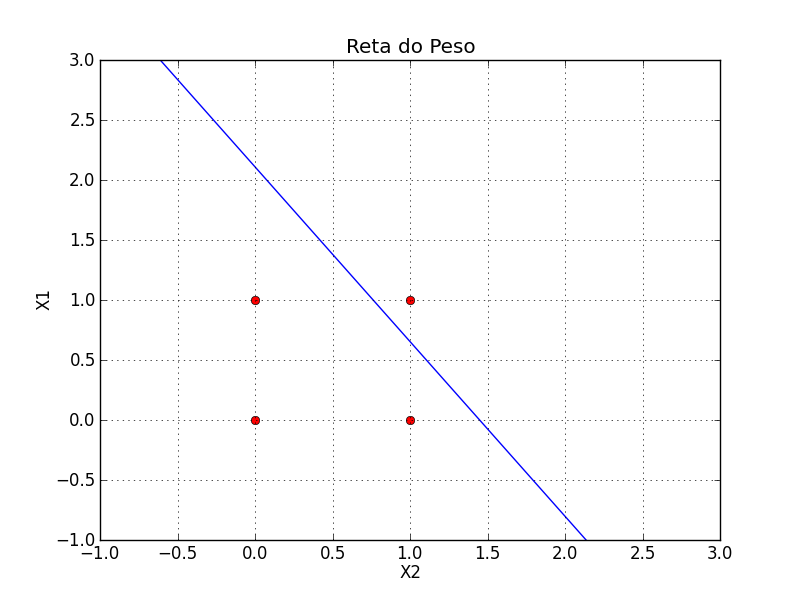
\includegraphics[width=0.70\textwidth]{C:/Users/LEONARDO/Desktop/Perceptron/arquivos/PessoAND.png}
	\caption{Reta de Decisão AND}
\end{figure}

\begin{figure}
	\centering
	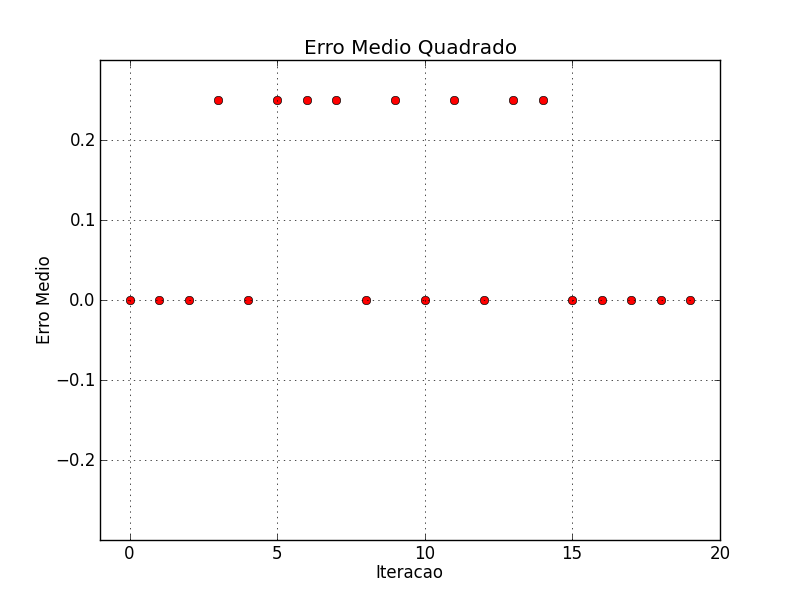
\includegraphics[width=0.70\textwidth]{C:/Users/LEONARDO/Desktop/Perceptron/arquivos/ErroAND.png}
	\caption{Erros do AND}
\end{figure}

\section{Separação de Duas Classes Bidimensionais}

Neste problema foi criado uma classe gauss que encapsulo a função gaussclass. Essa função recebe os números padrões que são as quantidade das amostras, a media e o desvio padrão que é um valor escalar. 

A função tem como objetivo criar duas classes e realizar o treinamento no perceptron, para isso primeiramente cria uma matriz aleatória usando a função random.randn, sendo a quantidade de linhas igual ao tamanha da dimensão das medias obtida pela função len e as colunas sendo igual a quantidade de números padrões, obtendo uma matriz x. 

No segundo momento usando a função tile que faz a replicação de matriz. Neste caso a função replica a matriz medias pela quantidade de números padrões obtendo uma matriz m.

No terceiro momento temos a obtenção da distribuição gaussiana, que com a matriz m, somada com o desvio padrão que é multiplica por x, obtemos a matriz da classe. Na figura 3 é possível visualizar duas classes bem definidas uma com media 1 e outro com a media 6 e desvio padrão 0,5.    

def gaussclass(self,numeropadroes, medias, desviopadrao):

\setlength{\parindent}{1,5 cm}
dimensao = len(medias)

x = random.randn(dimensao, numeropadroes) 

m = tile(medias, numeropadroes)  

classe = m + desviopadrao*x  

return classe

\setlength{\parindent}{1,0 cm}

Com a função montada e funcionando, foram construídas duas classes a e b, introduzida no perceptron para treinamento e obtenção de algumas informações. 

Primeiro teste:\\
quantidade de amostras (números padrões) = 100\\
media classe a = 1\\
media classe b = 6\\
desvio padrão = 0.5

Resultados:\\
quantidade de iterações 400 utilizadas de 10000 possíveis\\
vetor peso = [-0.03713852 -0.00679008 -0.11217314]\\
porcentagem de validação = 100\%

Conforme a figura 3 e valores inseridos no teste, obtemos uma representação de amostras sem superposição, consequentemente obtendo uma porcentagem de validação de 100 \%. Na figura 4 com os erros, percebe-se que os valores convergem para o ponto zero. \\ 

\begin{figure}
	\centering
	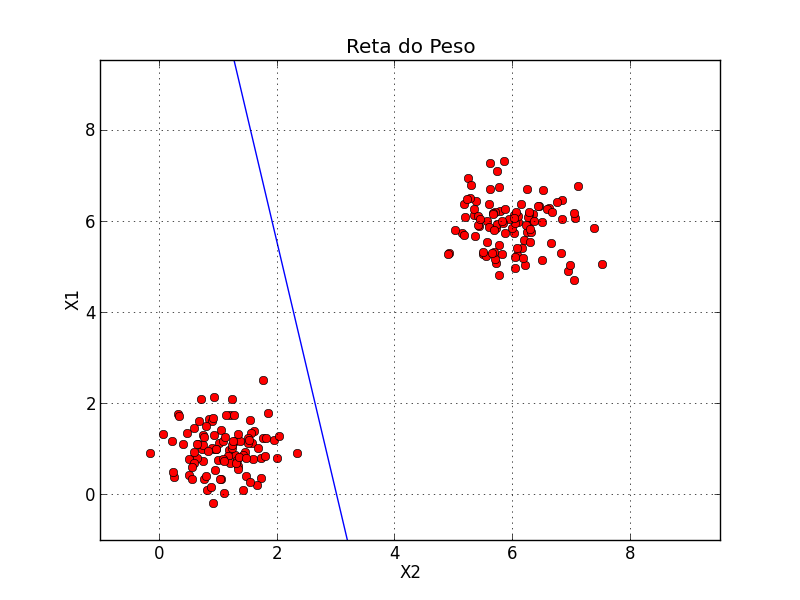
\includegraphics[width=0.70\textwidth]{C:/Users/LEONARDO/Desktop/Perceptron/arquivos/Pessosem.png}
	\caption{Reta de decisão sem Superposição}
\end{figure}

\begin{figure}
	\centering
	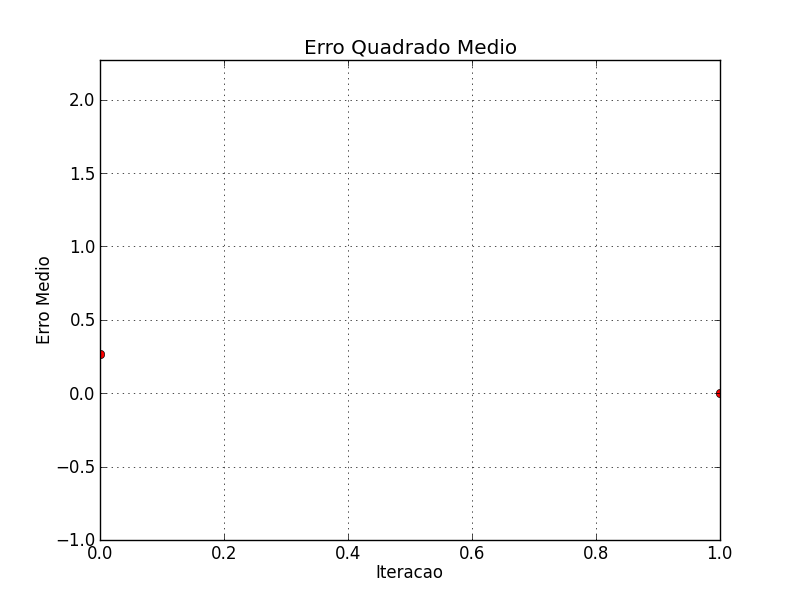
\includegraphics[width=0.70\textwidth]{C:/Users/LEONARDO/Desktop/Perceptron/arquivos/Errosem.png}
	\caption{Erros sem Superposição}
\end{figure}

Segundo teste:\\
quantidade de amostras = 30\\
media classe a = 1\\
media classe b = 3\\
desvio padrão = 1\\
Resultados:\\
quantidade de iterações 10000 utilizadas de 10000 possiveis\\
vetor peso  [-0.09859769 -0.08484054 -0.32790642]\\
porcentagem de validação 93\%\\

No segundo teste conforme a figura 5 e valores inseridos, temos um gráfico com superposição, onde não teve uma divisão da reta de decisão bem definida. Portanto não foi encontrado um teimamento com perfeição, obtendo uma porcentagem de validação igual á 95\%. Na figura 6 onde temos o gráfico de erro com superposição percebe-se que o valor não converge para o ponto zero. 

\begin{figure}
	\centering
	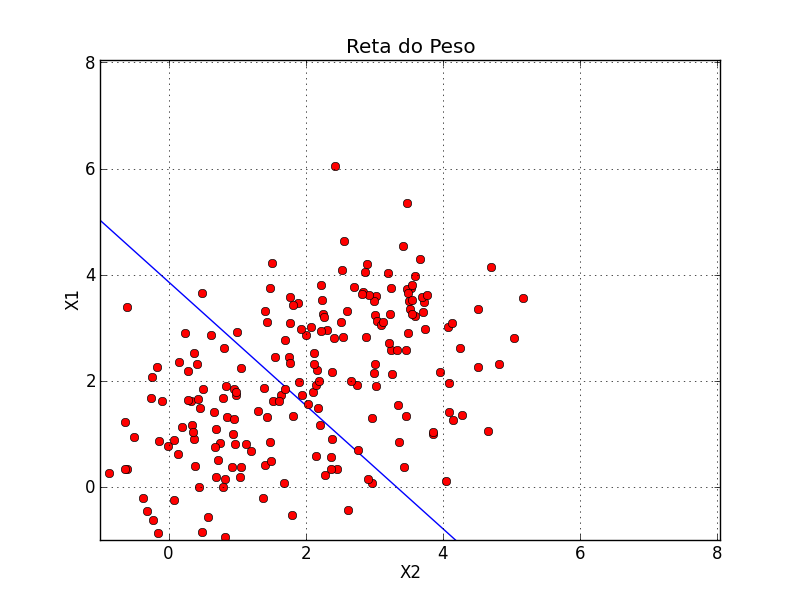
\includegraphics[width=0.70\textwidth]{C:/Users/LEONARDO/Desktop/Perceptron/arquivos/Pessocom.png}
	\caption{Reta de decisão com Superposição}
\end{figure}

\begin{figure}
	\centering
	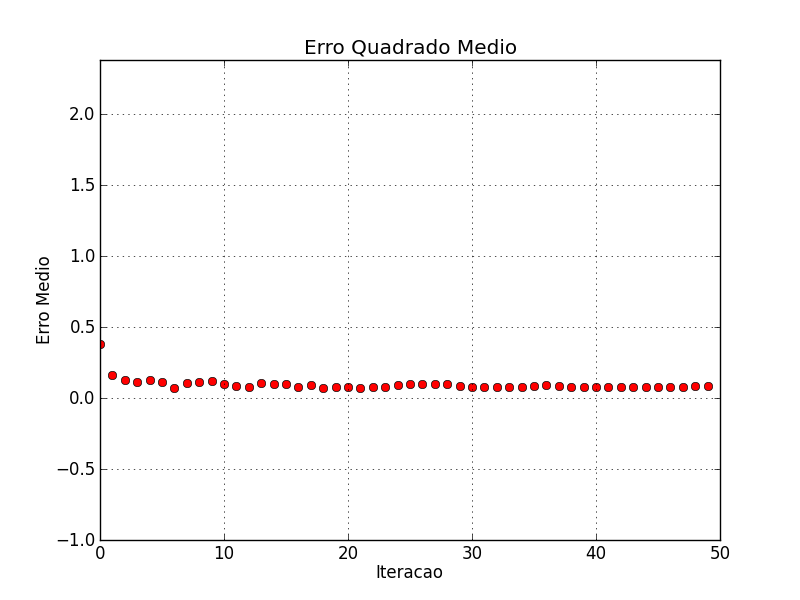
\includegraphics[width=0.70\textwidth]{C:/Users/LEONARDO/Desktop/Perceptron/arquivos/Errocom.png}
	\caption{Erros com Superposição}
\end{figure}

Fazendo uma analise geral dos dois testes onde se obtém um gráfico sem e com superposição. No primeiro conseguimos um treinamento perfeito e consequentemente obteremos respostas com 100\% de exatidão, já no segundo temos uma margem de erro, portanto suas repostas não e 100\% confiável.  

\section{Diagnóstico de Doença Cardíaca}

Neste problema foi realizado a conversão do algoritmo em matlab para python, não era necessário, simplesmente poderíamos pegar a função ordenada feita no matlab é inserir no perceptron que teríamos o resultado. Mas para maior aprendizagem foi realizado a conversão do algorítimo.     

A função dadosheart foi encapsula na classe heart. Com o objetivo bem simples, ordenar as amostras que estão inseridas no arquivo heart.txt, sendo que cada linha representa uma amostra e cada coluna um parâmetro ou tipo de variável. 

Primeiramente usando a função loadtxt que leu o arquivo heart.txt retornando uma matriz com valores de tipo float. No segundo momento com a função argsort ordenamos em ordem crescente  a matriz com relação a ultima coluna. No terceiro momento usando a função de transporta (dados.T), colocamos as amostras como coluna e os parâmetros como linha. 

Com a matriz encontrada e usando a manipulação de matrizes conforme mostrado no algoritmo, separamos as amostras e os valores esperados, salvos nas variáveis entrada e valord respectivamente. Com a entrada e o valor desejado encontrado, será possível fazer o treinamento do perceptron e consequentemente a obtenção de alguns resultados.     
  
def dadosheart(self):    
\setlength{\parindent}{1,5 cm}

heart = open("arquivos/heart.txt", "r")

dados = loadtxt("arquivos/heart.txt") 

heart.close()

dados = dados[dados[:,-1].argsort(),] 

dados = array(dados)

dados = dados.T

valord = dados[len(dados)-1, 0:(len(dados[0]))]-1

entrada = dados[0:len(dados)-1, 0:(len(dados[0]))]

self.entrada = array(entrada)

self.valord = array(valord)

print self.entrada
  
Com as funções montadas forma feitas dois testes:

\begin{figure}
	\centering
	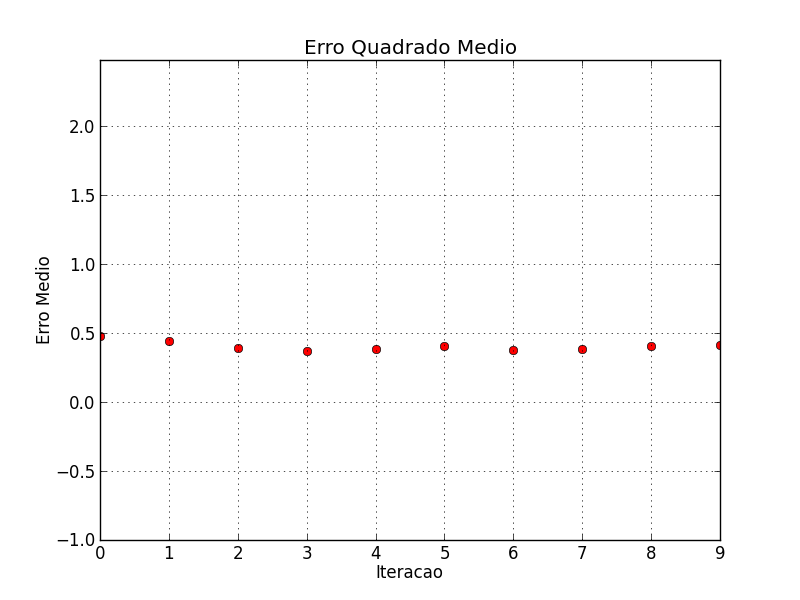
\includegraphics[width=0.70\textwidth]{C:/Users/LEONARDO/Desktop/Perceptron/arquivos/Erro10.png}
	\caption{Erros com 10 épocas}
\end{figure}

Primeiro teste:\\
quantidade repetições = 10\\
quantidade de iterações 2700 utilizadas de 2700 possíveis\\
Vetor Peso = [  4.12138123   1.99181923   4.71531328   2.52252534   3.33388862 -0.3170514    2.04987036  -9.11626037   2.09561386   4.02306266 2.27790664   4.79291722  11.88554654   0.03627629]\\
Porcentagem de validação 68,15\%\\

\begin{figure}
	\centering
	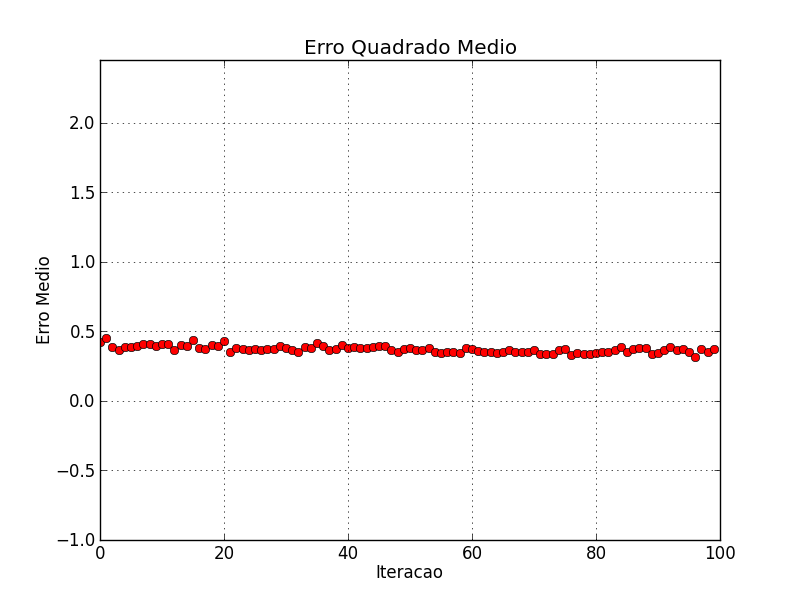
\includegraphics[width=0.70\textwidth]{C:/Users/LEONARDO/Desktop/Perceptron/arquivos/Erro100.png}
	\caption{Erros com 100 épocas}
\end{figure}

Segundo teste:\\
Quantidade repetições 100\\
Quantidade de iterações 27000 possíveis 27000\\
Vetor Peso = [ -2.06696215  13.18404771  37.90040708   6.83751641   0.13787567 -1.74000957   9.63414429 -12.18863627  13.22327649  28.97465394 6.16479329  36.00941059  74.09761003  -0.41615471]\\
Porcentagem de validação = 54,82\%\\

\begin{figure}
	\centering
	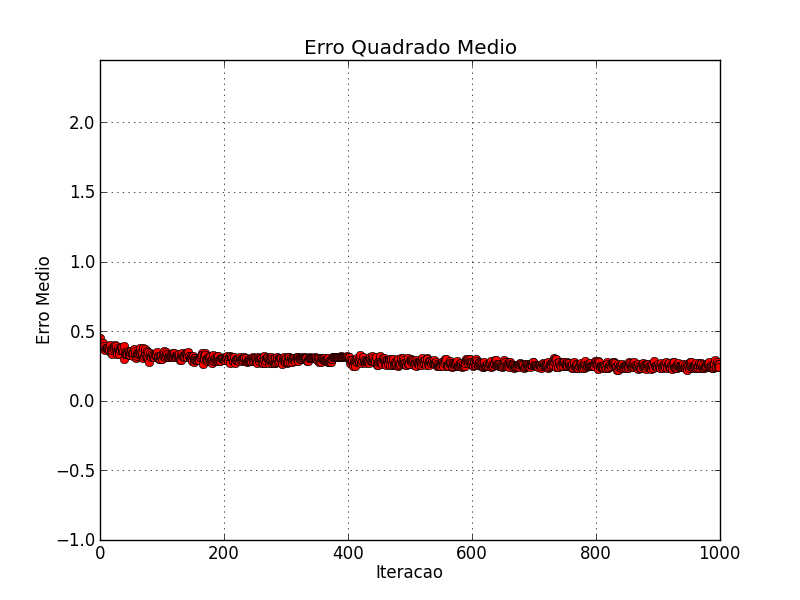
\includegraphics[width=0.70\textwidth]{C:/Users/LEONARDO/Desktop/Perceptron/arquivos/Erro1000.png}
	\caption{Erros com 1000 épocas}
\end{figure}

Terceiro teste:
Quantidade repetições 1000\\
Quantidade de iterações 270000 possíveis 270000\\
Vetor Peso = [ -12.69054951   90.28683129  161.75270871    3.45798984    0.49142011 -14.71468608  107.50227373  -12.73719681   56.53483721 103.75127108 42.33852524  234.01263772  172.29743844    6.65143898]\\
Porcentagem de validação = 86\%\\

No primeiro teste obtemos a figura 7 e no segundo obtemos a figura 8. Nos gráficos apresentados não dá para ter um visualização clara, devido a função ploterro no perceptron plotar todos os erros obtidos, que foram respectivamente 2700 e 27000 amostras de erro para 10 e 100 repetições. E para termos a visualiação bem definida devemos fazer a simulação no algoritmo e usar a ferramente de zoom apos a plotagem do gráfico.

Com os resultados obtidos vimos que o erro não converge para valor zero, provavelmente as amostras contém superposição, portanto tivemos um valor de validação com melhor resultado de 68,15\%. Mostrando que não precisa de uma quantidade grande de treinamentos para obter um resultado satisfatório. 

No terceiro teste obtivemos um resultado interessante, a porcentagem de validação ficou em torno de 86\%, e conforme a figura 9 onde temos o gráfico do erro, percebe-se que o valor está convergindo para zero. Neste teste fiz com 1000 repetições, sendo que foi muito demorado e não tentei com um valor maior, mas com esse teste possamos até pensar que o valor possa convergir à zero e ter uma validação de 100\%. Contrariando os resultados obtidos anteriormente realizado no mesmo problema, onde dava uma ideia de amostras com superposição. Portanto não podemos concluir sem fazer mais testes com uma maior quantidades de repetições. 

Por fim conforme pedido no trabalho foi criado um script geral de execução que recebe todas as classes montadas como uma biblioteca e executa de forma iterativa os dois problemas com a inserção de algumas informações.  
 
Como a implementação do perceptron, função dadosheart em python pode ser utilizada para várias dimensões e amostras. Portanto pode-se inserir outros tipos de amostras e parâmetros que a função dadosheart irá resolver.

\chapter*[CONCLUSÃO]{CONCLUSÃO}
\addcontentsline{toc}{chapter}{CONCLUSÃO}

A implementação do perceptron trouxe uma grande aprendizagem na linguagem Python e no funcionamento da rede perceptron, que talvez não obtivesse somente através de livros e resolução de exercícios, claro que para a implementação foi necessário o estudo do perceptron e o algoritmo python para realização do trabalho. Inicialmente o entendimento da rede perceptron não foi fácil, mas com o estudo bem elaborado é árduo percebe-se que o conteúdo não é difícil

O trabalho também exigiu o relatório na plataforma Látex, que também não foi fácil, porém gratificante por ter aprendido mais uma ferramenta, claro que preciso aprofundar ainda mais, mas já deu para aprender o básico. \cite{latex}\cite{latex2}

Uma percepção que obtive nos estudos de quando se visualizava um resolução de algum exemplo do perceptron, o aprendizado ficou enriquecedor, portanto como sugestão pedido no trabalho, talvez seria interessante a resolução em sala de aula de pelos menos um exercício.  

\bibliographystyle{abbrv}
\addcontentsline{toc}{section}{Bibliografia}
\bibliography{refs}
\end{document}


